The results shown in this section are obtained in standard fRG using an interaction cutoff: $G_0^\Lambda = \Lambda G_0$. The calculations are performed on the Matsubara frequency axis for temperature $T=0,08 t$, where $t$ is the nearest neighbors hopping.  

Besides the vertex, we have computed the susceptibilities, whose divergences follow the vertex ones. 

\subparagraph{Technicalities}

The vertex was decomposed in channels (magnetic, density, and superconducting) as usual in the literature. 

We have previously shown that the full frequency dependence of the vertex can change drastically the resutls (as opposed for example to a bosonic frequency transfer decomposition), and hence we kept all the frequencies in a finite box. 

The momentum dependence of the vertex is treated by means of a form factor decomposition, while keeping 29 patches in the respective bosonic momentum transfer . The critical scale is fixed by the condition that the absolute value of one of the channels exceeds a value of 300$D$, $D=4t$. 


In all the calculations in this section we did not include any self-energy feedback. The calculation of the self-energy, with a full frequency dependence vertex turned out to be problematic (for the standard fRG), and is ongoing work. 
 
 
\subparagraph{Results} 

In Fig \ref{phasediag_van_hove} and \ref{phasediag_van_hove_plus} we show  a putative phase diagram, for, respectively, van Hove filling, and van Hove filling plus 7\%. 

The fininte temperature acts as a cutoff for divergencies in the bare bubble. 

\begin{figure}
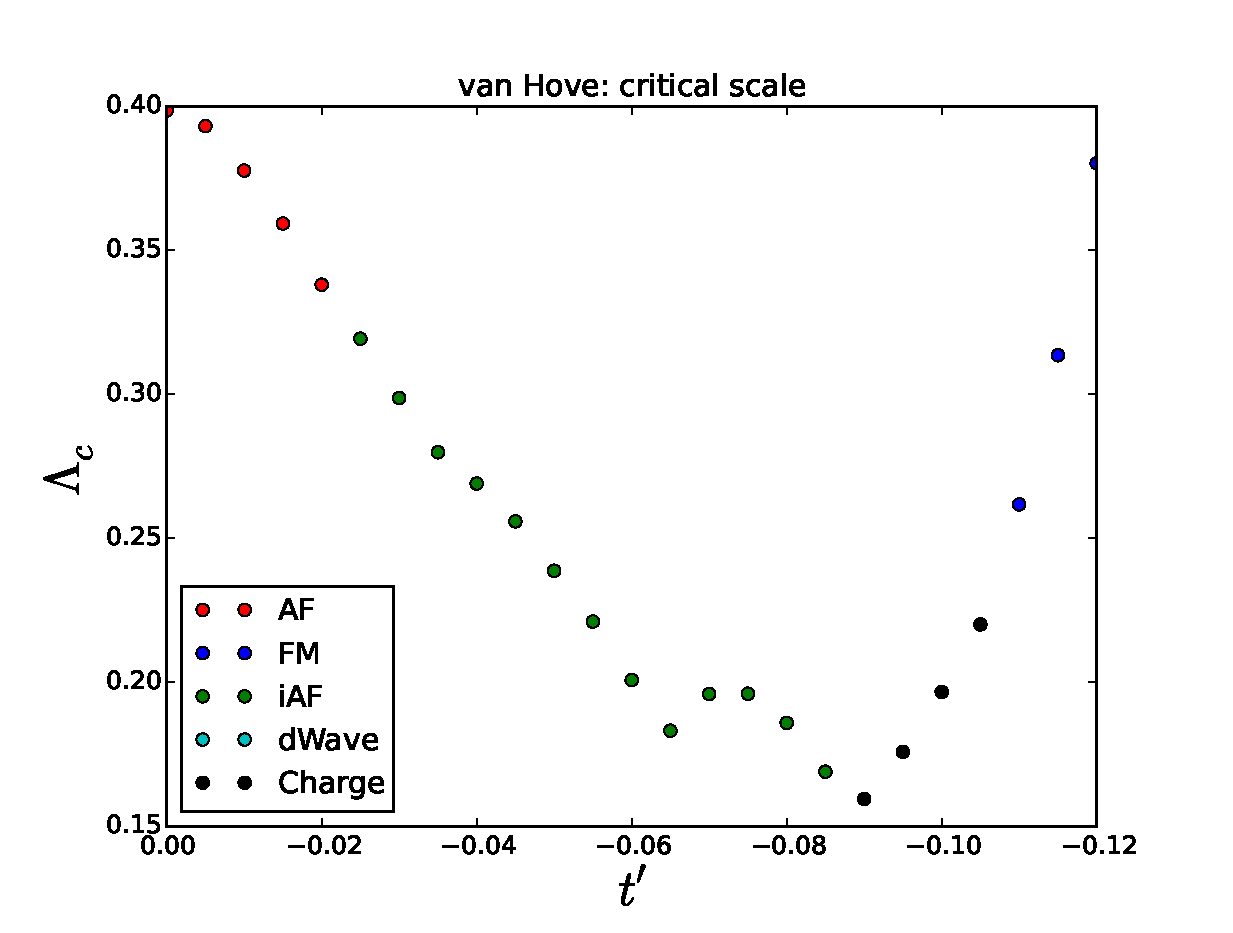
\includegraphics[scale=0.8]{vanHove_scan_critical_lambda_phi.eps}
\caption{Critical scale in full frequency fRG (interaction cutoff) as a function of the nearest neighbors hopping and for van Hove filling. The color of the symbol indicates the kind of instability that is realized.  } \label{phasediag_van_hove}

\end{figure}

\begin{figure}
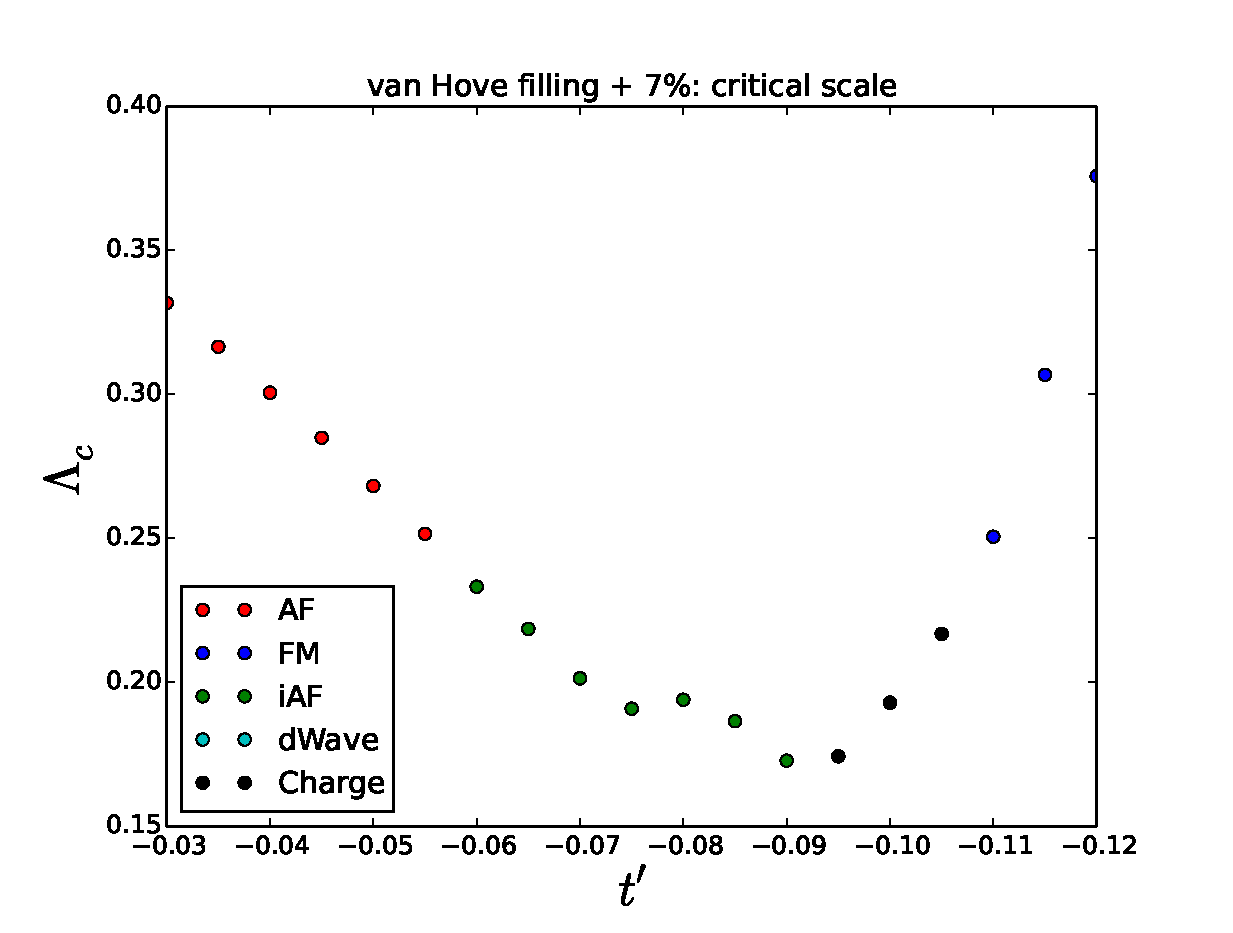
\includegraphics[scale=0.8]{vanHove_plus_scan_critical_lambda_phi.eps}
\caption{Critical scale in full frequency fRG (interaction cutoff) as a function of the nearest neighbors hopping and for van Hove filling + 7 \% . The color of the symbol indicates the kind of instability that is realized.} 
\label{phasediag_van_hove_plus} 
\end{figure}

In the spirit of the "interaction cutoff" the critical scale can be associated with the maximal value of the interaction $U_{\mathrm{flow}}\approx(1-\Lambda)^2 U$ \textbf{check if there is the square} for which the flow would converge. 
In a purely weak coupling scenario one can assume a monothonic relation between the interaction value and the critical temperature, and hence we can qualitatively associate the critical scale whith a critical temperature. In this sense our results are consistent with those reported in the literature. 

We hava double-checked the consistency of our results by also considering a frequency selective cuffoff, which substitutes: $i\omega \rightarrow i\mathrm{sign} \omega \sqrt{\omega^2+\Lambda^2}$. 

\begin{figure}
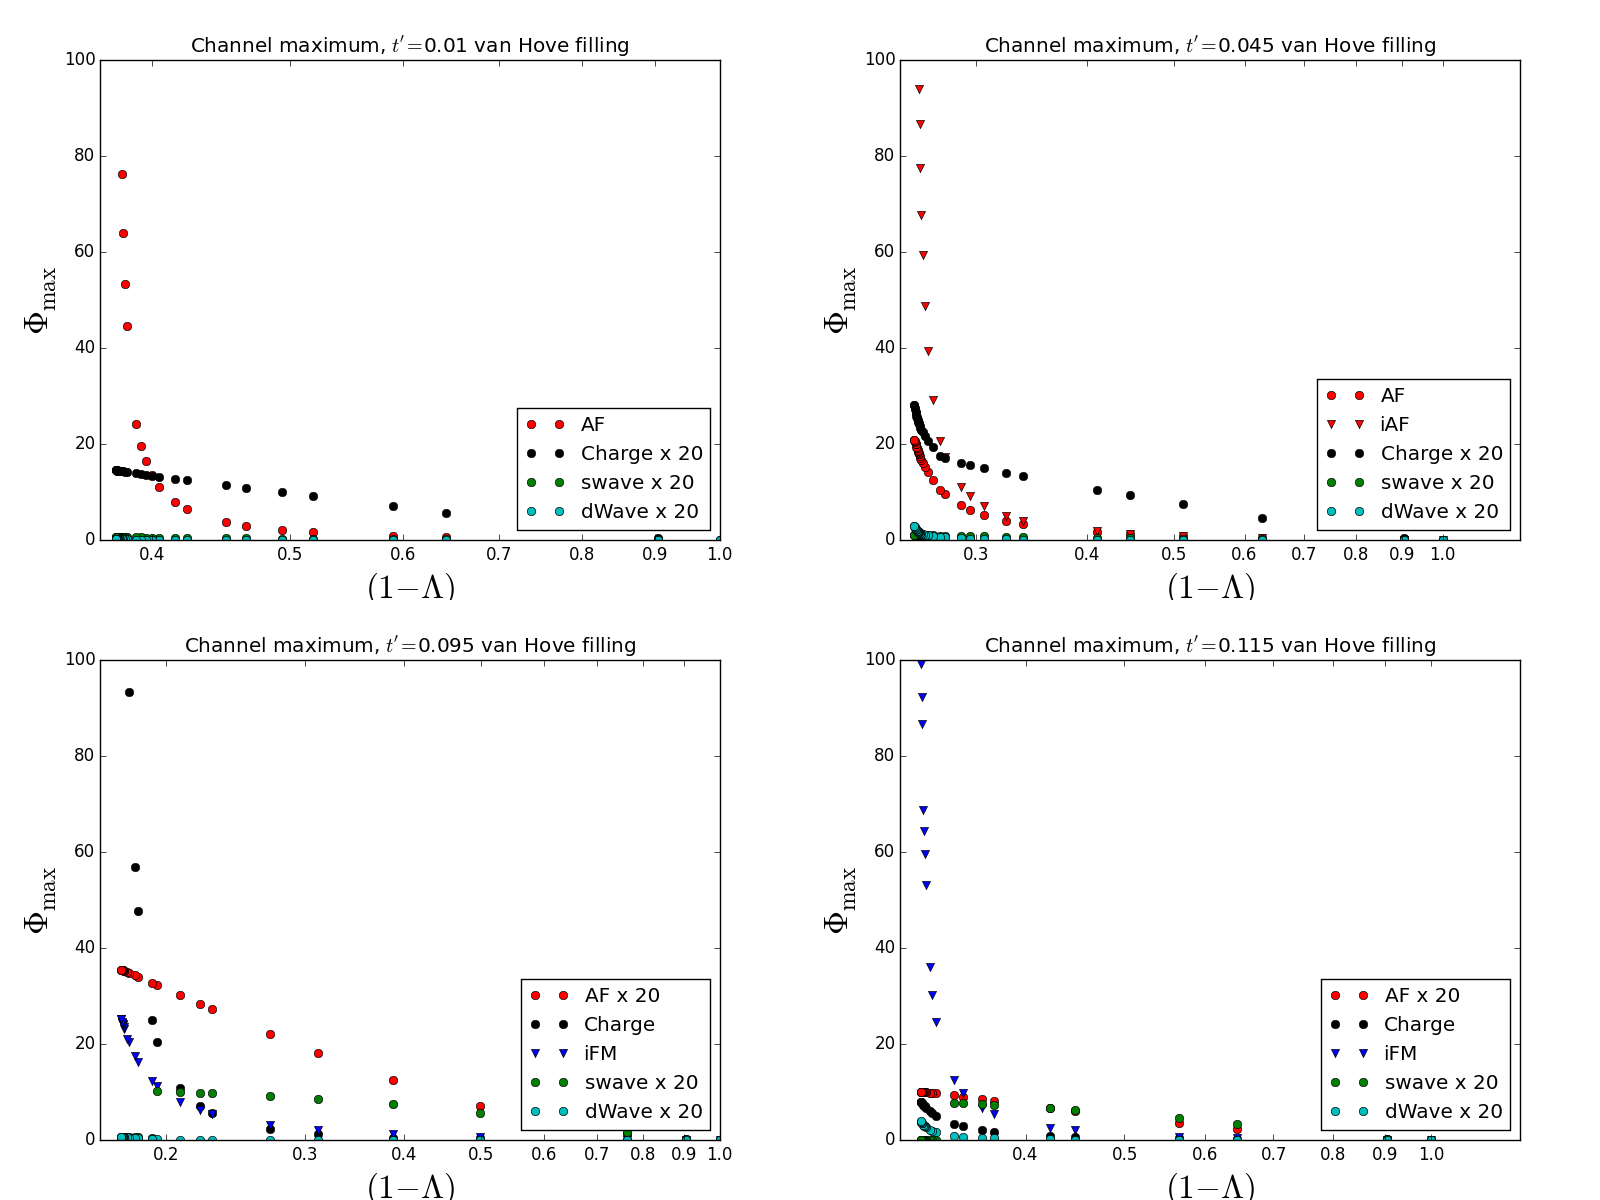
\includegraphics[scale=0.25]{images/vanhovelam.png}
\caption{Flow of the maximum of the absolute value of each channel for differnt values of $t'$ and at van Hove filling.
} 
\label{lamvan} 
\end{figure}

\begin{figure}
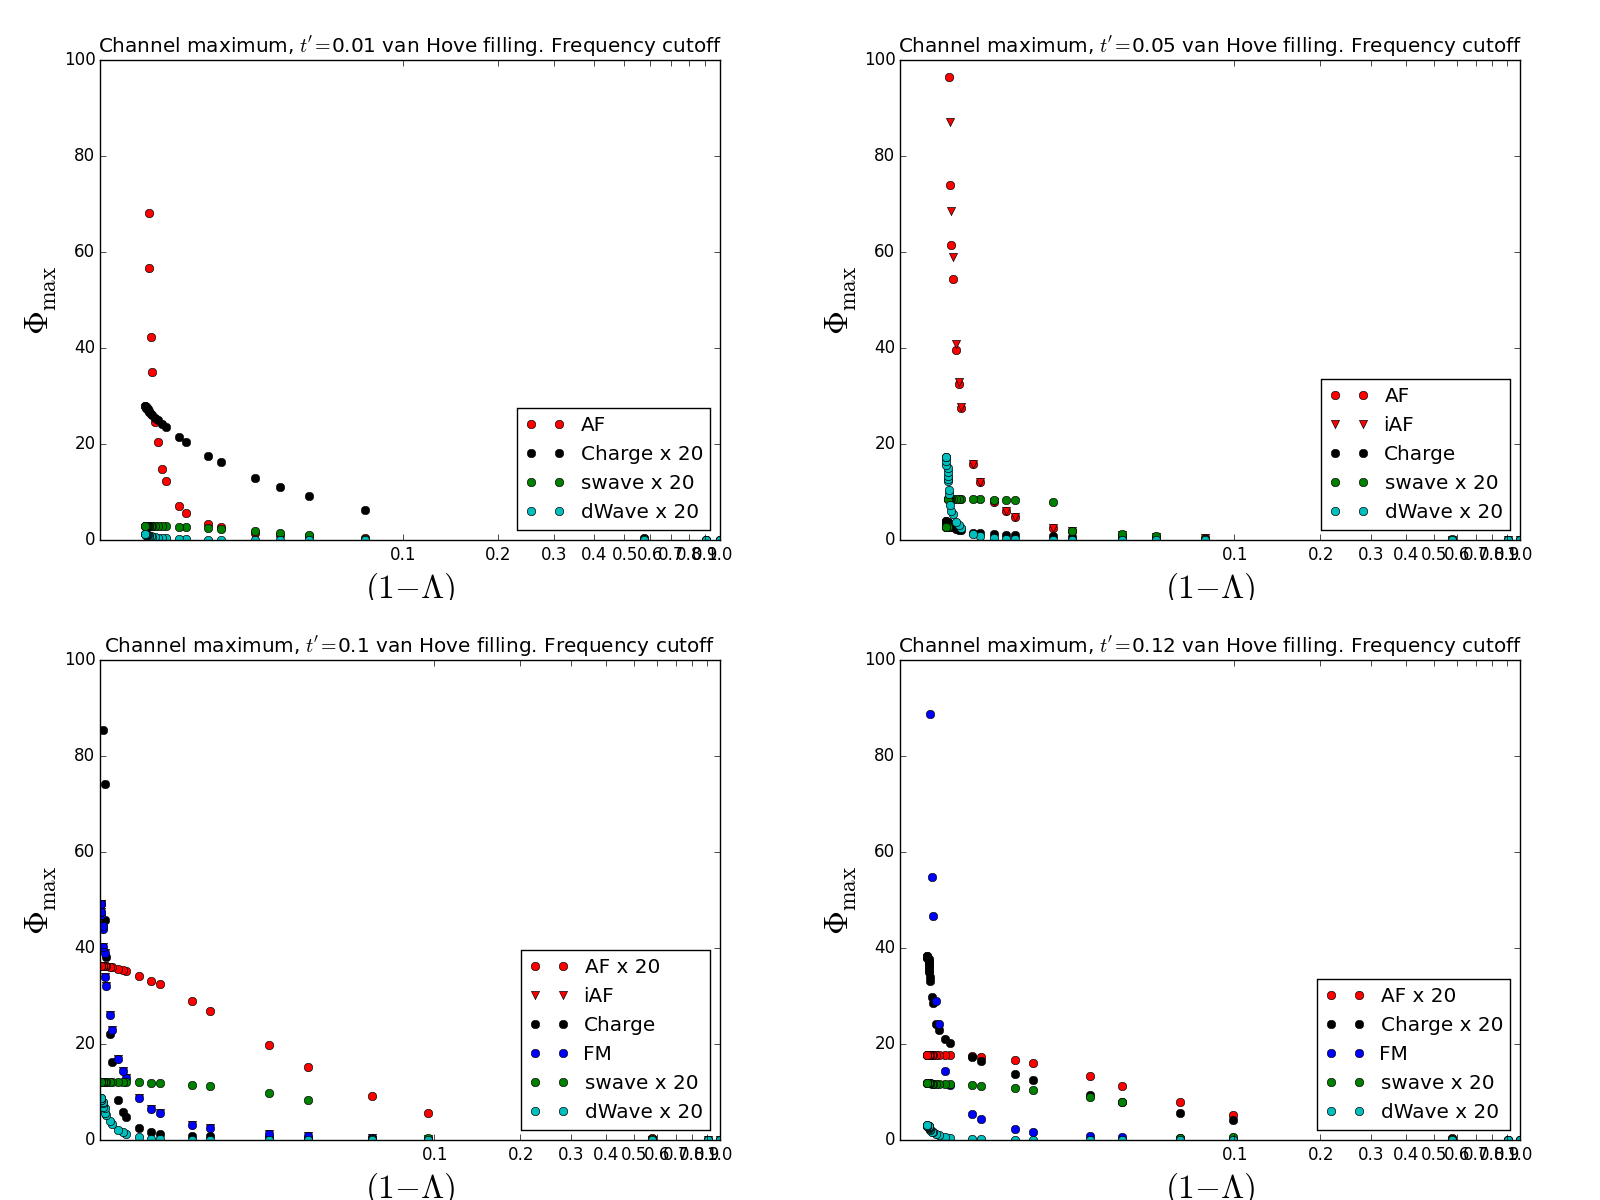
\includegraphics[scale=0.25]{images/freqvanhove.png}
\caption{Flow of the maximum of the absolute value of each channel for differnt values of $t'$ and at van Hove filling. } 
\label{freqlam} 
\end{figure}

\begin{figure}
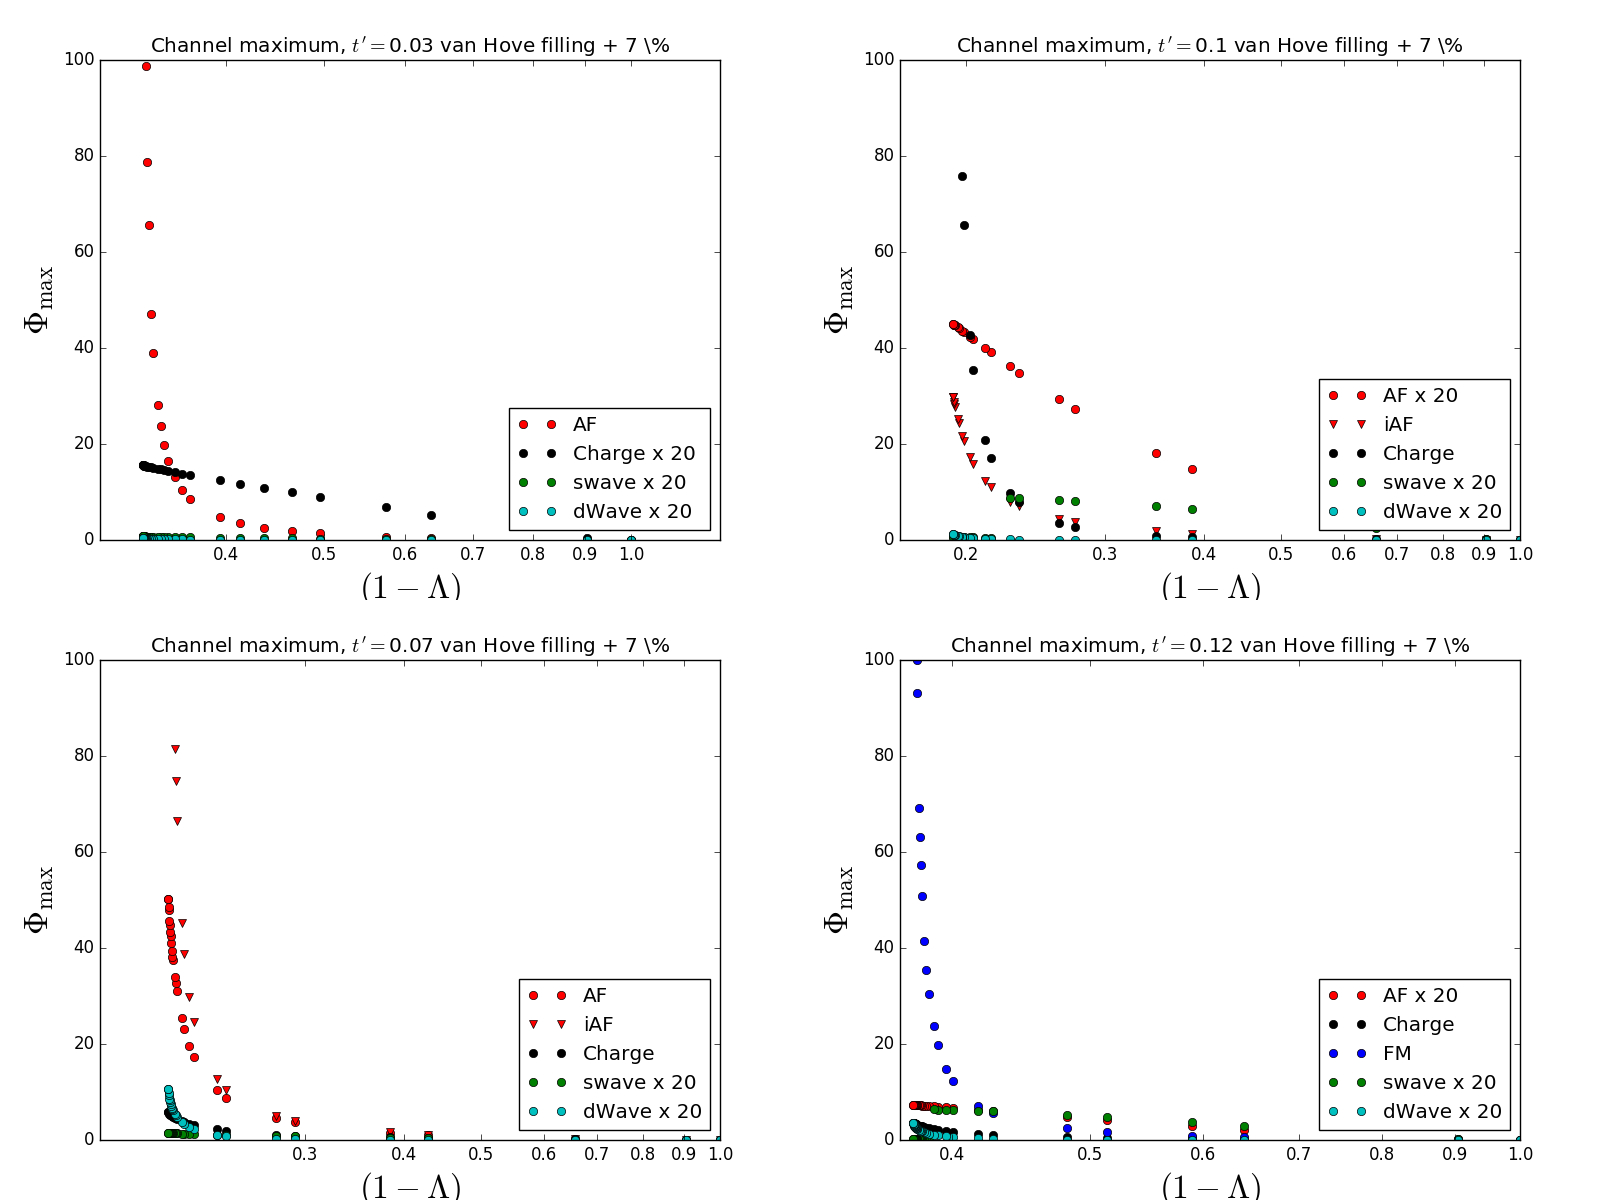
\includegraphics[scale=0.25]{images/vanhovepluslambda.png}
\caption{Flow of the maximum of the absolute value of each channel for differnt values of $t'$ and at van Hove filling $+7 \%$.
} 
\label{lamvanplus} 
\end{figure}

\subparagraph{Charge instability problem}

We call \textit{charge instability problem} the divergence of the charge component of the vertex for a finite bosonic frequency transfer, i.e. $\Omega_{ph} = 2\pi/\beta$, as already reported in the literature by Husemann \emph{et al}. 
\begin{itemize}
\item The charge channel diverges for a region of filling/next neighbors hopping between iAF and FM. In static fRG in this region one can find $d$wave superconductivity, usually at much lower scales. 
\item The \textit{divergence} of the channel is associated with a very specific \textit{frequency-structure}. The frequency-structure can be explainated (section about perpendicular ladders), it's divergence instead is unphysical. 
\item The charge-channel divergence arises also in DMF$^2$RG, where the DMFT self-energy is already included in the flow equations. 
\item Introducing a \emph{full} self-energy feedback the in DMF$^2$RG the problem seems to be suppressed. 
\item Similar observations in fRG, with major approximations on the self energy feedback.
\item The divergence is very localized in frequency space. Nevertheless it is sufficient to induce large values of the charge susceptibility, with a maximum at finite frequency transfer.    
\end{itemize} 
 
\textbf{Here include some color plots of the charge channel vs magnetic channel}

